\BourbakiBackSection{HISTORICAL NOTE}

(Numbers in brackets refer to the bibliography at the end of this note.)

The ideas of limit and continuity go back to antiquity, and a complete history of them could not be written without studying systematically from this point of view not only the Greek mathematicians but also the Greek philosophers and Aristotle in particular. It would also be necessary to trace the evolution of these ideas through Renaissance mathematics and the beginnings of the differential and integral calculus. Such a study, though it would undoubtedly be interesting to undertake, would go far beyond the framework of this note.

It is Riemann who should be considered as the creator of topology, as of so many other branches of modern mathematics. He was the first to attempt to formulate the notion of a topological space; he conceived the idea of an autonomous theory of such spaces; he defined invariants (the ``Betti numbers'') which were to play a pre-eminent part in the later development of topology; and he was the first to apply topology to analysis (periods of abelian integrals). But the current of ideas in the first half of the nineteenth century had prepared the path for Riemann in more ways than one. In the first place, the desire to put mathematics on a firm basis, which was the cause of so many important researches throughout the nineteenth century and up to the present day, had led to a correct understanding of the notions of a convergent series and a sequence of numbers tending to a limit (Cauchy, Abel) and to the notion of a continuous function (Bolzano, Cauchy). On the other hand, the geometrical representation (by points of a plane) of the complex numbers (or, as they had hitherto been called, ``imaginary'' or even ``impossible'' numbers) which was due to Gauss and Argand, had become familiar to the majority of mathematicians; it constituted an advance of the same order as the adoption, in our century, of the language of geometry in the study of Hilbert space, and contained the germ of the possibility of a geometrical representation of every object capable of continuous variation. Gauss, who was in any case naturally led to such concepts by his researches on the foundations of geometry, on non-Euclidean geometry and on curved surfaces, seems to have had this possibility already in mind, for he uses the words ``magnitude twice extended'' when defining (independently of Argand and the French mathematicians) the geometrical representation of complex numbers ({[}1{]}, pp.~101-103 and 175-178).

Riemann's work on algebraic functions and their integrals and his reflections on the foundations of geometry (largely inspired by his study of Gauss's work) led him to formulate a program of study, which is precisely that of modern topology, and to begin to realize this program. Here, for example, is what he says in his theory of abelian functions ({[}2{]}, p.~91):

``In the study of functions obtained by integrating exact differentials, some theorems of Analysis situs are almost indispensable. By this name, which was used by Leibnitz, although perhaps in a somewhat different sense, should be called that part of the theory of continuous magnitudes which studies these magnitudes, not independently of their position and by measuring them in terms of each other, but rather by abstracting all ideas of measurement and considering only their relations of position and inclusion. I reserve to a later occasion an investigation completely independent of all measurement\ldots{}''

And in his famous inaugural lecture ``On the hypotheses which underlie Geometry'' ({[}2{]}, p.~272):

``\ldots{} the general concept of a magnitude many times extended (*) which contains as a particular case that of spatial magnitude, has remained completely unexplored\ldots'' (p.~272)

``\ldots{} The notion of magnitude presupposes that an element is capable of different determinations. According as one can pass from one determination to another by a continuous process of transition or not, these determinations form a continuous or a discrete manifold: in the former case the determinations are called points of the manifold\ldots'' (p.~273)

``\ldots{} Measurement consists of superposition of the magnitudes to be compared, hence in order to measure we need some means of using one magnitude as a yardstick for another. In the absence of this we can compare two magnitudes only if one is part of the other\ldots{} The investigations which can be undertaken in this context form a part of the theory of magnitudes which is independent of the theory of measurement and in which the magnitudes are considered not as existing independently of their position nor as expressible in terms of a unit of measurement, but as regions in a manifold. Such investigations have become necessary in several parts of mathematics, in particular in the theory of many-valued analytic functions\ldots'' (p.~274)

``\ldots{} The determination of position in a given manifold, whenever this is possible, can be reduced to a finite number of numerical determinations. There are however manifolds in which the determination of position requires not a finite number but an infinite sequence or even a continuous manifold of determinations of magnitudes. For example, the possible determinations of a function on a given domain, or the possible forms of a spatial figure, give manifolds of this type.'' (p.~276)

Note in this last phrase the first idea of a study of functional spaces; Riemann had already expressed the same idea in his dissertation: ``the totality of these functions'', he stated in connection with the minimal problem known as Dirichlet's principle, ``forms a connected domain which is closed in itself'' ({[}2{]}, p.~30); this, though imperfectly expressed, is nevertheless the germ of the proof which Hilbert was later to give of Dirichlet's principle, and of most of the applications of function spaces to the calculus of variations.

As we have said, Riemann began the execution of this grandiose program by defining the ``Betti numbers'', first for a surface ({[}2{]}, pp.~92-93) and later ({[}2{]}, pp.~479-482; cf.~also {[}3{]}) for a manifold of any dimension, and applied this definition to the theory of integrals; for this and for the considerable development of this theory since Riemann's time we refer the reader to the Historical Notes to the chapters on algebraic topology in this series of volumes.

Before a general theory of topological spaces, such as Riemann had envisaged, could be developed, it was necessary that the theory of real numbers, of sets of numbers, of sets of points on a line, in a plane and in space should be more systematically investigated than they had been in Riemann's time. Such investigations were related on the other hand to research into the nature of irrational numbers (semi-philosophical by Bolzano and essentially mathematical by Dedekind) and to progress in the theory of functions of a real variable in which Riemann himself made an important contribution by his definition of the integral and his theory of trigonometrical series, and to which du Bois-Reymond, Dini and Weierstrass, among others, contributed; they were the work of the second half of the nineteenth century, and especially the work of Cantor, who was the first to define (originally on the line, later in Euclidean space of n dimensions) the notions of point of accumulation, closed set, open set, perfect set, and obtained the essential results on the structure of these sets on the line (cf.~the Historical Note to Chapter IV). In this context, not only the works of Cantor {[}4{]} should be consulted, but also his extremely interesting correspondence with Dedekind {[}5{]}, where the idea of dimensionality as a topological invariant can be found clearly expressed. The later progress of the theory is traced in a semi-historical, semi-systematic form in Schoenflies' book {[}6{]}; by far the most important acquisition was the theorem of Borel-Lebesgue, namely the fact that every bounded closed subset of Euclidean \(n\) -space \(\mathbf{R}^n\) (cf.~Chapter VI, § 1) satisfies axiom (C \(^{''}\) ) of § 9 of this chapter (the theorem was first proved by Borel for a closed interval on the line and a countable family of open intervals covering it).

Cantor's ideas had originally met with vigorous opposition (cf.~the Historical Note to Book I, Chapters I-IV). At any rate his theory of point-sets on the line and in the plane was quickly made use of and disseminated by the French and German schools of function-theory (Jordan, Poincaré, Klein, Mittag-Leffler, and later Hadamard, Borel, Baire, Lebesgue, etc.); each of the early Borel treatises, in particular, contains an elementary exposition of this theory (see for example {[}7{]}). As these ideas spread, their possible application to sets, not of points but of curves or functions, began to be considered in various quarters, as witness the title ``On the limit curves of a variety of curves'' of a memoir by Ascoli in 1883 {[}8{]} and a communication by Hadamard to the congress of mathematicians at Zürich in 1896 {[}9{]}; all this is closely related to the introduction of ``line functions'' by Volterra in 1887 and to the creation of ``functional calculus'' or theory of functions in which the argument is a function (cf.~Volterra's book on functional analysis {[}10{]}). On the other hand, Hilbert's famous memoir {[}11{]}, in which, taking up Riemann's ideas again, he proved the existence of the minimum in Dirichlet's principle and inaugurated the ``direct method'' in the calculus of variations, showed clearly the importance of considering sets of functions in which the Bolzano-Weierstrass principle holds, that is to say in which every sequence has a convergent subsequence. Such sets were beginning in any case to play an important part, not only in the calculus of variations but also in the theory of functions of a real variable (Ascoli, Arzelà) and a little later in the theory of functions of a complex variable (Vitali, Carathéodory, Montel). Finally the study of functional equations, and especially the solution by Fredholm of the type of equation which bears his name, made it commonplace to consider a function as an argument and a set of functions as a set of points, and as natural to use the language of geometry in this context as in Euclidean space of \(n\) dimensions (a space which equally eludes ``intuition'' and for this reason remained long an object of distrust to many mathematicians). In particular the memorable work of Hilbert on integral equations {[}12{]} led to the definition and geometrical study of Hilbert space by Erhard Schmidt {[}14{]}, in complete analogy with Euclidean geometry.

Meanwhile the concept of an axiomatic theory had acquired more and more importance, thanks to much work on the foundations of geometry; here Hilbert's contributions {[}13{]} had a particularly decisive influence. In the course of this work, Hilbert had been led to formulate in 1902 ({[}13{]}, p.~180) the first axiomatic definition of the ``manifold twice extended'' in the sense of Riemann, a definition which constituted, said Hilbert, ``the foundation of a rigorous axiomatic treatment of Analysis situs''. Hilbert also made use of neighbourhoods (in a sense restricted by the demands of the problem to which he limited himself).

The first attempts to abstract what is common to properties of sets of points and sets of functions are due to Fréchet {[}15{]} and F. Riesz {[}16{]}. The former started from the notion of countable limit and did not succeed in constructing a convenient and fruitful system of axioms, but at least he recognized the relationship between the principle of Bolzano-Weierstrass {[}which is just axiom (C) of § 9, restricted to countable sequences{]} and the Borel-Lebesgue theorem {[}axiom (C'') of § 9{]}; in this connection he introduced the word ``compact'', although in a sense somewhat different from that in which it is used in this series of volumes. As to F. Riesz, who took as his starting point the concept of point of accumulation (or rather of ``derived set'', which amounts to the same thing), his theory was again incomplete and appeared only in outline form.

General topology as it is understood today began with Hausdorff ({[}17{]}, Chapters 7, 8, 9), who again took up the concept of neighbourhood (by which he meant what in the terminology of this series of volumes is called an ``open neighbourhood'') and chose from Hilbert's axioms for neighbourhoods in the plane those which gave his theory all the precision and generality desired. The axioms he took as a starting-point were essentially (taking into account the difference between his concept of neighbourhood and ours) axioms ( \(V_{I}\) ), ( \(V_{II}\) ), ( \(V_{III}\) ), ( \(V_{IV}\) ) of § I and (H) of § 8, and the chapter in which he develops the consequences of these axioms has remained a model of axiomatic theory, abstract but adapted in advance to applications. Hausdorff's work was naturally the point of departure for later research in general topology and especially for the work of the Moscow school, which was largely directed towards the problem of metrization (cf.~the Historical Note to Chapter IX); here we recall especially the definition of compact spaces (under the name of ``bicompact spaces'') by Alexandroff and Urysohn, and Tychonoff's proof of the compactness of products of compact spaces {[}19{]}. Finally, the introduction of filters by H. Cartan {[}20{]} has brought to topology a valuable instrument, usable in all sorts of applications (in which it replaces to advantage the notion of ``Moore-Smith convergence'' {[}18{]}). Furthermore, the development of the theorem on ultrafilters (Theorem 1, § 6), has clarified and simplified the theory.

\BourbakiBackSection{BIBLIOGRAPHY}

{[}1{]} C. F. GAUSS, Werke, Vol. 2, Göttingen, 1863.

{[}2{]} B. RIEMANN, Gesammelte mathematische Werke, 2nd edition, Leipzig (Teubner), 1892.

{[}3{]} B. RIEMANN, in Lettere di E. Betti a P. Tardy, Rend. Accad. Lincei (5) 24 \(^{1}\) (1915) pp.~517-519.

{[}4{]} G. CANTOR, Gesammelte Abhandlungen, Berlin (Springer), 1932.

{[}5{]} G. CANTOR and R. DEDEKIND, Briefwechsel, Actualités scientifiques et industrielles, no. 518, Paris (Hermann), 1937.

{[}6{]} A. SCHOENFLIES, Entwicklungen der Mengenlehre und ihrer Anwendungen, Part I, 2nd edition, Leipzig-Berlin (Teubner), 1913.

{[}7{]} E. BOREL, Leçons sur la théorie des fonctions, 2nd edition, Paris (Gauthier-Villars), 1914.

{[}8{]} G. Ascoli, Le curve limiti di una varietà data di curve, Mem. Accad. Lincei (3) 18 (1883) p.~521-586.

{[}9{]} J. HADAMARD, Sur certaines applications possibles de la théorie des ensembles, Verhandl. Intern. Math.-Kongress, Zürich, 1898, pp.~201-202.

{[}10{]} V. VOLTERRA, Theory of Functionals, London-Glasgow (Blackie and Son), 1930.

{[}11{]} D. HILBERT, Gesammelte Abhandlungen, vol.~3, Berlin (Springer), 1935, pp.~10-37 {[}= Jahresbericht des D.M.V., 8 (1900), p.~184, and Math. Ann., 59 (1904), p.~161{]}.

{[}12{]} D. HILBERT, Grundzüge einer allgemeinen Theorie der Integralgleichungen, 2nd edition, Leipzig-Berlin (Teubner), 1924.

{[}13{]} D. HILBERT, Grundlagen der Geometrie, 7th edition, Leipzig-Berlin (Teubner), 1930.

{[}14{]} E. SCHMIDT, Über die Auflösung linearer Gleichungen mit unendlich vielen Unbekannten, Rend. Palermo, 25 (1908), pp.~53-77.

{[}15{]} M. FRÉCHET, Sur quelques points du calcul fonctionnel, Rend. Palermo, 22 (1906), pp.~1-74.

{[}16{]} F. RIESZ, Stetigkeitsbegriff und abstrakte Mengenlehre, Atti del IV Congresso Intern. dei Matem., Bologna, 1908, vol.~2, pp.~18-24.

{[}17{]} F. HAUSDORFF, Grundzüge der Mengenlehre, 1st edition, Leipzig (Veit), 1914.

{[}18{]} E. H. MOORE and H. L. SMITH, A general theory of limits, Am. Journ. of Math., 44 (1922) pp.~102-121.

{[}19{]} A. TYCHONOFF, Über die topologische Erweiterung von Räumen, Math. Ann., 102 (1930), pp.~514-561.

{[}20{]} H. CARTAN, Théorie des filtres; filtres et ultrafiltres, C. R. Acad. Sc. Paris, 205 (1937), pp.~595-598 and pp.~777-779.

\chapter{Uniform Structures}

\section{UNIFORM SPACES}

\subsection{DEFINITION OF A UNIFORM STRUCTURE}

DEFINITION 1. A uniform structure (or uniformity) on a set X is a structure given by a set U of subsets of X × X which satisfies axioms (F\_I) and (F\_II) of Chapter I, § 6, no. 1 and also satisfies the following axioms:

\((\mathbf{U}_{\mathbf{I}})\) Every set belonging to \(\mathfrak{U}\) contains the diagonal \(\Delta\) .

\((\mathbf{U}_{\mathbf{II}})\) If \(\mathbf{V}\in \mathfrak{U}\) then \(\overline{\mathbf{V}}^1\in \mathfrak{U}\) .

\((\mathbf{U}_{\mathbf{III}})\) For each \(\mathbf{V} \in \mathfrak{U}\) there exists \(\mathbf{W} \in \mathfrak{U}\) such that \(\mathbf{W} \circ \mathbf{W} \subset \mathbf{V}\) .

\pandocbounded{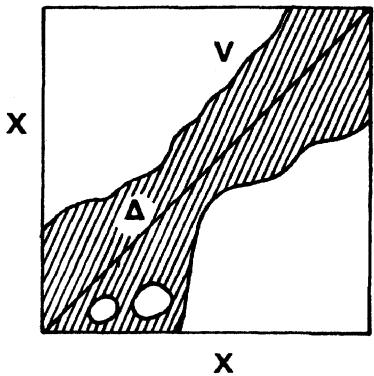
\includegraphics[keepaspectratio]{images/part001_6ce88dc6.jpg}}\\
Figure 2.

The sets of \(\mathfrak{U}\) are called entourages of the uniformity defined on \(\mathbf{X}\) by \(\mathfrak{U}\) . A set endowed with a uniformity is called a uniform space.

If V is an entourage of a uniformity on X, we may express the relation \((x, x') \in V\) by saying that ``x and \(x'\) are V-close''.

Remarks. 1) To make the language more expressive we may use the expressions ``x is close enough to y'' and ``x and y are as close as we please'' in some statements. For example, we shall say that a relation

R \(\{x,y\}\) is true whenever x and y are close enough if there is an entourage V such that the relation \((x,y)\in V\) implies R \(\{x,y\}\) .

\begin{enumerate}
\def\labelenumi{\arabic{enumi})}
\setcounter{enumi}{1}
\tightlist
\item
  The conjunction of axioms (U \(_{II}\) ) and (U \(_{III}\) ) is equivalent (assuming the other axioms of uniform structures) to the following axiom:
\end{enumerate}

\((\mathbf{U}_a)\) For each \(\mathbf{V} \in \mathfrak{U}\) there exists \(\mathbf{W} \in \mathfrak{U}\) such that \(\mathbf{W} \circ \overline{\mathbf{W}} \subset \mathbf{V}\) (*).

Clearly \((\mathbf{U}_{\mathrm{II}})\) and \((\mathbf{U}_{\mathrm{III}})\) imply \((\mathbf{U}_a)\) . Conversely, if \((\mathbf{U}_a)\) is satisfied we have \(\overline{\mathbf{W}} = \Delta \circ \overline{\mathbf{W}} \subset \mathbf{V}\) , by \((\mathbf{U}_I)\) ; hence \(\mathbf{W} \subset \overline{\mathbf{V}}\) and therefore {[}by \((\mathbf{F}_I)] \overline{\mathbf{V}} \in \mathfrak{U}\) . Let \(\mathbf{W}' = \mathbf{W} \cap \overline{\mathbf{W}}\) ; then \(\mathbf{W}' \in \mathfrak{U}\) by what has just been proved and axiom \((\mathbf{F}_{\mathrm{II}})\) , and we have \(\mathbf{W}' \circ \mathbf{W}' \subset \mathbf{W} \circ \overline{\mathbf{W}} \subset \mathbf{V}\) .

Throughout this chapter we shall write \(\mathbf{V}\) instead of \(\mathbf{V} \circ \mathbf{V}\) , and in general \(\mathbf{V} = \mathbf{V} \circ \mathbf{V} = \mathbf{V} \circ \mathbf{V}\) , for each integer \(n > 1\) and each subset \(\mathbf{V}\) of \(\mathbf{X} \times \mathbf{X}\) .

\begin{enumerate}
\def\labelenumi{\arabic{enumi})}
\setcounter{enumi}{2}
\tightlist
\item
  If X is not empty, then axiom \((U_{I})\) implies that no set of U is empty, and therefore U is a filter on \(X \times X\) . There is only one uniformity on the empty set, namely \(U = \{\varnothing\}\) .
\end{enumerate}

DEFINITION 2. A fundamental system of entourages of a uniformity is any set B of entourages such that every entourage contains a set belonging to B.

Axiom \((\mathbf{U}_{\mathbf{III}})\) shows that if n is any integer \textgreater0 and V runs through a fundamental system of entourages, then the sets \(V^{n}\) again form a fundamental system of entourages.

Entourages V such that \(V = \overline{V}^{1}\) are called symmetric. If V is any entourage, then \(V \cap \overline{V}^{1}\) and \(V \cup \overline{V}^{1}\) are symmetric entourages, and axioms \((F_{\mathrm{II}})\) and \((U_{\mathrm{II}})\) show that the symmetric entourages form a fundamental system of entourages.

A set \(\mathfrak{B}\) of subsets of \(\mathbf{X} \times \mathbf{X}\) is a fundamental system of entourages of a uniformity on \(\mathbf{X}\) if and only if \(\mathfrak{B}\) satisfies axiom ( \(B_{\mathbf{I}}\) ) of Chapter I, § 6, no. 3, and also satisfies the following axioms:

\((\mathbf{U}_{\mathbf{I}}^{\prime})\) Every set of \(\mathfrak{B}\) contains the diagonal \(\Delta\) .

\((\mathbf{U}_{\mathbf{II}}^{\prime})\) For each \(\mathbf{V} \in \mathfrak{B}\) there exists \(\mathbf{V}' \in \mathfrak{B}\) such that \(\mathbf{V}' \subset \overline{\mathbf{V}}^1\) .

\((\mathbf{U}_{\mathbf{III}}^{\prime})\) For each \(\mathbf{V} \in \mathfrak{B}\) there exists \(\mathbf{W} \in \mathfrak{B}\) such that \(\tilde{\mathbf{W}} \subset \mathbf{V}\) .

If X is not empty, a fundamental system of entourages of a uniform structure on X is a base of the filter formed by the entourages of this structure (Chapter I, § 6, no. 3, Proposition 3).

(*) We recall (Set Theory, R, § 3, nos. 4 and 10) that if V and W are two subsets of \(\mathbf{X} \times \mathbf{X}\) , then the set of pairs \((x, y) \in \mathbf{X} \times \mathbf{X}\) , such that \((x, z) \in \mathbf{W}\) and \((z, y) \in \mathbf{V}\) for some \(z \in \mathbf{X}\) , is denoted by V o W or VW, and that the set of pairs \((x, y) \in \mathbf{X} \times \mathbf{X}\) such that \((y, x) \in \mathbf{V}\) is denoted by \(\overline{\mathbf{V}}\) .

Examples of uniformities. * 1) On the set R of real numbers we can define a uniformity, called the additive uniformity, as follows: for each \(\alpha > 0\) let \(V_{\alpha}\) be the subset of \(R \times R\) consisting of all pairs \((x, y)\) such that \(|x - y| < \alpha\) ; as \(\alpha\) runs through the set of all real numbers \(> 0\) , the \(V_{\alpha}\) form a fundamental system of entourages for the additive uniformity on R. Similarly we can define a uniformity (again called the additive uniformity) on the set Q of rational numbers; we shall study these structures, and analogous uniform structures on groups, in Chapters III and IV. * 2) Let X be a set and let R be an equivalence relation on X; let C be

the graph of R in \(\mathbf{X} \times \mathbf{X}\) . Then \(\Delta \subset \mathbf{C}\) and \(\tilde{\mathbf{C}} = \tilde{\mathbf{C}} = \mathbf{C}\) ; (Set Theory, R, § 5, no. 1); the set of subsets of \(\mathbf{X} \times \mathbf{X}\) which consists of the set C alone is therefore a fundamental system of entourages of a uniformity on X. In particular, if we take R to be the relation of equality, then \(\mathbf{C} = \Delta\) and the entourages of the corresponding uniformity are all the subsets of \(\mathbf{X} \times \mathbf{X}\) which contain \(\Delta\) ; this uniformity is called the discrete uniformity on X, and the set X endowed with this uniformity is called a discrete uniform space.

\begin{enumerate}
\def\labelenumi{\arabic{enumi})}
\setcounter{enumi}{2}
\tightlist
\item
  On the set \(\mathbf{Z}\) of rational integers we can define a uniformity, important in the theory of numbers, as follows: given a prime number \(p\) , let \(\mathbf{W}_n\) be the set of all pairs \((x,y)\in \mathbf{Z}\times \mathbf{Z}\) such that \(x\equiv y\) (mod \(p^n\) ), for each integer \(n > 0\) . It is easily verified that the sets \(\mathbf{W}_n\) (for a fixed \(p\) ) form a fundamental system of entourages of a uniformity on \(\mathbf{Z}\) , called the \(p\) -adic uniformity (cf.~Chapter III, § 6, Exercises 23 ff., and Chapter IX, § 3, no. 2).
\end{enumerate}

In accordance with the general definitions (Set Theory, R, § 8, no. 5), if X and X' are two sets each endowed with uniformities whose sets of entourages are U and U' respectively, then a bijection f of X onto X' is an isomorphism of the uniformity of X onto that of X' if g(U) = U', where g = f × f.

For example, if X and \(X'\) are two equipotent sets, then every bijection of X onto \(X'\) is an isomorphism of the discrete uniformity of X onto the discrete uniformity of \(X'\) .

\subsection{TOPOLOGY OF A UNIFORM SPACE}

PROPOSITION 1. Let X be a set endowed with a uniform structure U, and for each \(x \in X\) let \(\mathfrak{B}(x)\) be the set of subsets \(\mathbf{V}(x)\) of \(\mathbf{X}(*)\) , where V runs through the set of entourages of U. Then there is a unique topology on X such that, for each \(x \in X\) , \(\mathfrak{B}(x)\) is the neighbourhood filter of x in this topology.

We have to show that the \(\mathfrak{B}(x)\) satisfy conditions \((\mathbf{V}_{\mathbf{I}})\) , \((\mathbf{V}_{\mathbf{II}})\) , \((\mathbf{V}_{\mathbf{III}})\) and \((\mathbf{V}_{\mathbf{IV}})\) of Chapter I, § 1, no. 2. That this is so for the first three of these conditions follows immediately from the fact that the entourages of \(\mathcal{U}\) satisfy \((\mathbf{F}_{\mathbf{I}})\) , \((\mathbf{F}_{\mathbf{II}})\) and \((\mathbf{U}_{\mathbf{I}})\) . As to \((\mathbf{V}_{\mathbf{IV}})\) , let \(\mathbf{V}\) be an entourage of \(\mathcal{U}\) , \(\mathbf{W}\) an entourage of \(\mathcal{U}\) such that \(\hat{\mathbf{W}} \subset \mathbf{V}\) ; then if \((x, y) \in \mathbf{W}\) and \((y, z) \in \mathbf{W}\) we have \((x, z) \in \mathbf{V}\) , so that \(\mathbf{W}(y) \subset \mathbf{V}(x)\) for all \(y \in \mathbf{W}(x)\) , and therefore \(\mathbf{V}(x) \in \mathfrak{B}(y)\) for all \(y \in \mathbf{W}(x)\) . This completes the proof.

DEFINITION 3. The topology defined in Proposition 1 is called the topology induced by the uniform structure U.

Examples. * 1) The topology induced by the additive uniformity on the set of real numbers is the topology of the real line (Chapter I, § 1, no. 2); similarly the topology induced by the additive uniformity on the set of rational numbers is the topology of the rational line. *

\begin{enumerate}
\def\labelenumi{\arabic{enumi})}
\setcounter{enumi}{1}
\tightlist
\item
  On any set X, the topology induced by the discrete uniformity (no. 1, Example 2) is the discrete topology.
\end{enumerate}

In the future, when we speak of the topology of a uniform space X, we shall always mean the topology induced by the uniform structure of the space, unless the contrary is expressly stated. The topological space obtained by putting this topology on the set X is sometimes called the topological space underlying the uniform space in question. For example, when we say that a uniform space is Hausdorff, or compact, or locally compact, etc., we mean that the underlying topological space has this property.

If X and \(X'\) are two uniform spaces, any isomorphism f of the uniform structure of X onto that of \(X'\) is also a homeomorphism of X onto \(X'\) ; we say that X is an isomorphism of the uniform space X onto the uniform space \(X'\) . It should be noted that a homeomorphism of X onto \(X'\) is not necessarily an isomorphism of the uniform structure of X onto that of \(X'\) .

\pandocbounded{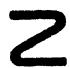
\includegraphics[keepaspectratio]{images/part001_037a61a5.jpg}}

In other words, distinct uniformities on the same set X can induce the same topology. * For example, on {]}0, +∞{[}, the additive and the multiplicative uniformities (which are distinct : Chapter III, § 6, Exercise 17) induce the same topology. *

For another example see § 2, no. 2, Remark 1.

PROPOSITION 2. Let X be a uniform space. For every symmetric entourage V of X and every subset M of X × X, VMV is a neighbourhood of M in the product space X × X, and the closure of M in this space is given by the formula

\[
\overline {{\mathbf {M}}} = \bigcap_ {\mathbf {V} \in \mathfrak {S}} \mathbf {V M V}\tag{I}
\]

where \(\mathfrak{S}\) denotes the set of symmetric entourages of \(\mathbf{X}\) .

Let V be a symmetric entourage of X. The relation \((x, y) \in \text{VMV}\) means that there is an element \((p, q)\) of M such that \((x, p) \in V\) and \((q, y) \in V\) : in other words (V being symmetric) \(x \in V(p)\) and \(y \in V(q)\) , that is \((x, y) \in V(p) \times V(q)\) . Since \(V(p) \times X(q)\) is a neighbourhood of \((p, q)\) in \(X \times X\) , the first part of the proposition is proved. The relations \((x, p) \in V\) , \((y, q) \in V\) can also be written \(p \in V(x)\) , \(q \in V(y)\) or \((p, q) \in V(x) \times V(y)\) . As V runs through S, the sets \(V(x) \times V(y)\) form a fundamental system of neighbourhoods of \((x, y)\) in \(X \times X\) ; for if U, \(U'\) are any two entourages there is always a symmetric entourage \(V \subset U \cap U'\) , so that \(V(x) \times V(y) \subset U(x) \times U'(y)\) . Hence \(V(x) \times V(y)\) meets M for each \(V \in S\) if and only if \((x, y) \in \overline{\mathbf{M}}\) , and formula (1) follows.

COROLLARY 1. If A is any subset of X and V is any symmetric entourage of X, then V(A) is a neighbourhood of A in X, and

\[
\overline {{{\mathbf {A}}}} = \bigcap_ {\mathbf {v} \in \mathfrak {S}} \mathbf {V} (\mathbf {A}) = \bigcap_ {\mathbf {v} \in \mathfrak {U}} \mathbf {V} (\mathbf {A})\tag{2}
\]

where \(\mathfrak{U}\) denotes the set of all entourages in \(\mathbf{X}\) .

If \(\mathbf{M} = \mathbf{A} \times \mathbf{A}\) , then \(\mathrm{VMV} = \mathrm{V}(\mathbf{A}) \times \mathrm{V}(\mathbf{A})\) for any \(\mathbf{V} \in \mathfrak{S}\) ; for the relation ``there exists \(p \in \mathbf{A}\) such that \((x, p) \in \mathbf{V}"\) is by definition equivalent to \(x \in \mathbf{V}(\mathbf{A})\) . The corollary now follows from Chapter I, § 4, no. 2, Proposition 5 and no. 3, Proposition 7.

V(A) is said to be the V-neighbourhood of A.

If V is an entourage which is open in X × X, then V(x) is open in X for each x ∈ X (Chapter I, § 4, no. 2, Corollary to Proposition 4) and therefore V(A), being the union of the V(x) as x runs through A, is open in X. On the other hand, if V is a closed entourage in X × X, V(A) need not be closed in X for every subset A of X (Exercise 3).

\pandocbounded{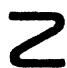
\includegraphics[keepaspectratio]{images/part001_f8cd4ad5.jpg}}

It should also be remarked that as V runs through the set of entourages of X, the sets V(A) do not necessarily form a fundamental system of neighbourhoods of A in X (Exercise 2).

COROLLARY 2. The interiors (resp. the closures) of the entourages of X in X × X form a fundamental system of entourages of X.

If V is any entourage of X, there is a symmetric entourage W such that \(W \subset V\) ; since W is a neighbourhood of W (Proposition 2), the interior of V in \(X \times X\) contains W and is therefore an entourage. Furthermore, we have \(W \subset W \subset W \subset V\) by Proposition 2, and hence V contains the closure of an entourage.

COROLLARY 3. Every uniform space satisfies axiom (O \(_{III}\) ).

If \(x\) is any point of \(X\) and \(V\) runs through the entourages of \(X\) which are closed in \(X \times X\) , then the sets \(V(x)\) form a fundamental system of neighbourhoods of \(x\) in \(X\) by Corollary 2, and they are closed in \(X\) (Chapter I, § 4, no. 2, Corollary to Proposition 4).

PROPOSITION 3. A uniform space X is Hausdorff if and only if the intersection of all the entourages of its uniform structure is the diagonal \(\Delta\) of \(X \times X\) . Every Hausdorff uniform space is regular.

The latter statement follows immediately from Corollary 3 to Proposition 2. We have seen that the closed entourages form a fundamental system of entourages (Proposition 2, Corollary 2); if their intersection is \(\Delta\) , then \(\Delta\) is closed in \(X \times X\) and consequently \(X\) is Hausdorff (Chapter I, § 8, no. 1, Proposition 1). Conversely, if \(X\) is Hausdorff then for every point \((x, y) \notin \Delta\) there is an entourage \(V\) of \(X\) such that \(y \notin V(x)\) , or equivalently \((x, y) \notin V\) ; hence \(\Delta\) is the intersection of all the entourages.

If a uniform space X is Hausdorff, we say that the uniform structure of X is Hausdorff. If B is a fundamental system of entourages for this structure; then X is Hausdorff if and only if the intersection of all the sets of B is \(\Delta\) .

\section{UNIFORMLY CONTINUOUS FUNCTIONS}

\subsection{UNIFORMLY CONTINUOUS FUNCTIONS}

DEFINITION 1. A mapping \(f\) of a uniform space \(\mathbf{X}\) into a uniform space \(\mathbf{X}'\) is said to be uniformly continuous if, for each entourage \(\mathbf{V}'\) of \(\mathbf{X}'\) , there is an entourage \(\mathbf{V}\) of \(\mathbf{X}\) such that the relation \((x,y)\in \mathbf{V}\) implies \((f(x),f(y))\in \mathbf{V}'\) .

In more expressive terms we may say that \(f\) is uniformly continuous if \(f(x)\) and \(f(y)\) are as close to each other as we please whenever \(x\) and \(y\) are close enough.

If we put \(g = f \times f\) , then Definition 1 means that whenever \(V'\) is an entourage of \(X'\) , \(\overline{g}^1(V')\) is an entourage of \(X\) .

Examples. 1) The identity mapping of a uniform space onto itself is uniformly continuous.

\begin{enumerate}
\def\labelenumi{\arabic{enumi})}
\setcounter{enumi}{1}
\item
  A constant mapping of a uniform space into a uniform space is uniformly continuous.
\item
  Every mapping of a discrete uniform space into a uniform space is uniformly continuous.
\end{enumerate}

PROPOSITION 1. Every uniformly continuous mapping is continuous.

This is an immediate consequence of the definitions.

On the other hand, a continuous mapping of a uniform space X into a uniform space \(X'\) need not be uniformly continuous, * as is shown by the example \(x \to x^{3}\) , a homeomorphism of R onto itself, which is not uniformly continuous with respect to the additive uniformity. * (See § 4, no. 1, Theorem 2.)

PROPOSITION 2. (a) If \(f: \mathbf{X} \to \mathbf{X}'\) and \(g: \mathbf{X}' \to \mathbf{X}''\) are two uniformly continuous mappings, then \(g \circ f: \mathbf{X} \to \mathbf{X}''\) is uniformly continuous.

\begin{enumerate}
\def\labelenumi{(\alph{enumi})}
\setcounter{enumi}{1}
\tightlist
\item
  A bijection \(f\) of a uniform space \(\mathbf{X}\) onto a uniform space \(\mathbf{X}'\) is an isomorphism if and only if \(f\) and the inverse of \(f\) are uniformly continuous.
\end{enumerate}

This follows immediately from the interpretation of Definition 1 in terms of the product mapping \(f \times f\) .

\subsection{COMPARISON OF UNIFORMITIES}

Proposition 2 of no. 1 shows that we can take as morphisms of uniform structures the uniformly continuous mappings (Set Theory, Chapter IV, § 2, no. 1); we shall always assume in the future that the morphisms have been so chosen. In accordance with the general definitions (Set Theory, Chapter IV, § 2, no. 2), this allows us to define an order relation on the set of uniformities on a given set X:

DEFINITION 2. If \(\mathfrak{U}_1\) and \(\mathfrak{U}_2\) are two uniform structures on the same set \(\mathbf{X}\) , \(\mathfrak{U}_1\) is said to be finer than \(\mathfrak{U}_2\) (and \(\mathfrak{U}_2\) coarser than \(\mathfrak{U}_1\) ) if, denoting by \(\mathbf{X}_i\) the set \(\mathbf{X}\) with the uniform structure \(\mathfrak{U}_i\) ( \(i = 1,2\) ), the identity mapping \(\mathbf{X}_1 \to \mathbf{X}_2\) is uniformly continuous.

If \(\mathfrak{U}_1\) is finer than \(\mathfrak{U}_2\) and distinct from \(\mathfrak{U}_2\) , we say that \(\mathfrak{U}_1\) is strictly finer than \(\mathfrak{U}_2\) (and that \(\mathfrak{U}_2\) is strictly coarser than \(\mathfrak{U}_1\) ).

Two uniformities are said to be comparable if one is finer than the other.

Example. In the ordered set of uniformities on a set X, the discrete uniformity is the finest, and the coarsest uniformity is that in which the set of entourages consists of the single element \(X \times X\) .

The following proposition is an immediate consequence of Definition 1 of no. 1:

PROPOSITION 3. If \(\mathfrak{U}_1\) and \(\mathfrak{U}_2\) are two uniformities on a set \(X\) , then \(\mathfrak{U}_1\) is finer than \(\mathfrak{U}_2\) if and only if every entourage of \(\mathfrak{U}_2\) is an entourage of \(\mathfrak{U}_1\) .

COROLLARY. Let \(\mathfrak{U}_1\) and \(\mathfrak{U}_2\) be two uniformities on a set \(X\) , and suppose that \(\mathfrak{U}_1\) is finer than \(\mathfrak{U}_2\) ; then the topology induced by \(\mathfrak{U}_1\) is finer than the topology induced by \(\mathfrak{U}_2\) .

This follows immediately from the comparison of topologies in terms of neighbourhoods (Chapter I, § 2, no. 2, Proposition 3).

Remarks. 1) It can happen that a uniformity \(\mathcal{U}_1\) is strictly finer than a uniformity \(\mathcal{U}_2\) but that the two induced topologies are identical. The following example shows this:

Let \(\mathbf{X}\) be a non-empty set. For each finite partition \(\varpi = (\mathrm{A}_i)_{1\leqslant i\leqslant n}\) of \(\mathbf{X}\) , let \(\mathrm{V}_{\overline{\omega}}\) denote

\[
\bigcup_ {i} \mathrm{A} _ {i} \times \mathrm{A} _ {i}.
\]

The sets \(V_{\overline{w}}\) then form a fundamental system of entourages of a uniformity \(\mathcal{U}\) on \(X\) . For if \(\varpi\) is any finite partition of \(X\) we have \(\Delta \subset V_{\overline{w}}\) and \(V_{\overline{w}} \circ V_{\overline{g}} = \overline{V}_{\overline{w}}^{1} = V_{\overline{w}}\) (§ 1, no. 1, Example 2); and if \(\varpi' = (B_j)\) and \(\varpi'' = (C_k)\) are two finite partitions of \(X\) , then those of the sets \(B_j \cap C_k\) which are not empty form a finite partition \(\varpi\) of \(X\) , and we have \(V_{\overline{w}} \subset V_{\overline{w}'} \cap V_{\overline{w}''}\) . \(\mathcal{U}\) is called the uniformity of finite partitions on \(X\) . The topology induced by. \(\mathcal{U}\) is the discrete topology, since for each \(x \in X\) the sets \(\{x\}\) and \(C\{x\}\) form a finite partition of \(X\) . Nevertheless, if \(X\) is infinite, it is clear that \(\mathcal{U}\) is strictly coarser than the discrete uniformity. 2) If \(f: X \to X'\) is a uniformly continuous mapping, then \(f\) remains uniformly continuous if we replace the uniformity of \(X\) by a finer uniformity and that of \(X'\) by a coarser uniformity (no. 1, Proposition 2). In other words, the finer the uniformity of \(X\) and the coarser the uniformity of \(X'\) , the more uniformly continuous mappings there are of \(X\) into \(X'\) .

\subsection{INITIAL UNIFORMITIES}

PROPOSITION 4. Let X be a set, let \((\mathrm{Y}_{t})_{t\in I}\) be a family of uniform spaces, and for each \(t\in I\) let \(f_{t}\) be a mapping of X into \(Y_{t}\) . For each \(t\in I\) let \(g_{t}\) denote \(f_{t}\times f_{t}\) . Let S be the set of subsets of \(X\times X\) of the form \(\overline{g}_{t}(V_{t})\) , where \(t\in I\) and \(V_{t}\) is an entourage of \(Y_{t}\) , and let B be the set of all finite intersections

\[
\mathbf {U} \left(\mathrm{V} _ {\iota_ {1}}, \dots , \mathrm{V} _ {\iota_ {n}}\right) = _ {i} ^ {- 1} g _ {i} \left(\mathrm{V} _ {\iota_ {1}}\right) \cap \dots \cap^ {- 1} g _ {\iota_ {n}} \left(\mathrm{V} _ {\iota_ {n}}\right)\tag{1}
\]

of sets of \(\mathfrak{S}\) . Then \(\mathfrak{B}\) is a fundamental system of entourages of a uniformity \(\mathfrak{U}\) on \(\mathbf{X}\) which is the initial uniform structure on \(\mathbf{X}\) with respect to the family \((f_{\mathfrak{i}})\) (Set Theory, Chapter IV, § 2, no. 3), and in particular \(\mathfrak{U}\) is the coarsest uniformity on \(\mathbf{X}\) for which all the mappings \(f_{\mathfrak{i}}\) are uniformly continuous. But otherwise, let \(h\) be a mapping of a uniform space \(\mathbf{Z}\) into \(\mathbf{X}\) ; then \(h\) is uniformly continuous (when \(\mathbf{X}\) is endowed with the uniformity \(\mathfrak{U}\) ) if and only if each of the mappings \(f_{\mathfrak{i}} \circ h\) is uniformly continuous.

It is immediately seen that \(\mathfrak{B}\) satisfies axioms \((\mathbf{B}_1)\mathbf{Y}\) and \((\mathbf{U}_1')\) . If \(\mathbf{W}_t = \overline{g}_t^1 (\mathbf{V}_t)\) , then \(\overline{\mathbf{W}}_t = \overline{g}_t^1 (\overline{\mathbf{V}}_t^1)\) and \(\dot{\mathbf{W}}_t = \overline{g}_t^1 (\overline{\mathbf{V}}_t^2)\) ; hence \(\mathfrak{B}\) also satisfies axioms \((\mathbf{U}_{\mathrm{II}}^t)\) and \((\mathbf{U}_{\mathrm{III}}^t)\) and is therefore a fundamental system of entourages of a uniformity \(\mathcal{U}\) on \(\mathbf{X}\) . Furthermore, it follows immediately from the definition of \(\mathcal{U}\) and Definition 1 and no. 1 that \(f_{t}\) is uniformly continuous for each index \(i\in I\) ; hence (no. 1, Proposition 2) \(f_{t}\circ h\) is uniformly continuous for each \(i\in I\) if \(h\) is. Conversely, suppose that \(f_{t}\circ h\) is uniformly continuous for each \(i\in I\) , and consider a set \(\mathrm{U}(\mathrm{V}_{i_t},\dots,\mathrm{V}_{i_n})\) ; by hypothesis, for each \(k\) such that \(1\leqslant k\leqslant n\) , there is an entourage \(\mathbf{W}_k\) of \(\mathbf{Z}\) such that the relation \((z,z^{\prime})\in \mathbf{W}_k\) implies \([f_{i_k}(h(z)),f_{i_k}(h(z')))]\in \mathbf{V}_k\) ; if

\[
\mathbf {W} = \bigcap_ {k} \mathbf {W} _ {k},
\]

these \(n\) relations are simultaneously satisfied whenever \(z\) and \(z'\) are W-close, so that we have then \((h(z), h(z')) \in \mathrm{U}(\mathrm{V}_{\iota_1}, \ldots, \mathrm{V}_{\iota_n})\) , and the proof is complete.

COROLLARY. The topology on X induced by the coarsest uniformity U for which the \(f_{i}\) are uniformly continuous is also the coarsest topology for which the \(f_{i}\) are continuous.

This is an immediate consequence of the definition of the neighbourhoods of a point in this latter topology (Chapter I, § 2, no. 3, Proposition 4).

The general properties of initial structures (Set Theory, Chapter IV, § 2, no. 3, criterion CST 10) imply in particular the following transitivity property:

PROPOSITION 5. Let X be a set, let \((Z_{\iota})_{\iota \in I}\) be a family of uniform spaces, let \((J_{\lambda})_{\lambda \in L}\) be a partition of I and let \((Y_{\lambda})_{\lambda \in L}\) be a family of sets indexed by L. For each \(\lambda \in L\) , let \(h_{\lambda}\) be a mapping of X into \(Y_{\lambda}\) ; for each \(\lambda \in L\) and each \(\iota \in J_{\lambda}\) , let \(g_{\iota \lambda}\) be a mapping of \(Y_{\lambda}\) into \(Z_{\iota}\) ; and let \(f_{\iota} = g_{\iota \lambda} \circ h_{\lambda}\) . Let each \(Y_{\lambda}\) carry the coarsest uniform structure for which the mappings \(g_{\iota \lambda} (\iota \in J_{\lambda})\) are uniformly continuous. Then the coarsest uniform structure on X for which the \(f_{\iota}\) are uniformly continuous is the same as the coarsest uniform structure on X for which the \(h_{\lambda}\) are uniformly continuous.

\subsection{INVERSE IMAGE OF A UNIFORMITY; UNIFORM SUBSPACES}

Let X be a set, Y a uniform space, f a mapping of X into Y. The coarsest uniformity U on X for which f is uniformly continuous is called the inverse image under f of the uniform structure of Y. It follows from Proposition 4 of no. 3, and from the formulae which give the inverse image of an intersection, that the inverse images under \(g = f \times f\) of the entourages of Y form a fundamental system of entourages for U. The topology induced by U is the inverse image under f of the topology of Y (no. 3, Corollary to Proposition 4).

Remark. If \(f: \mathbf{X} \to \mathbf{Y}\) is surjective, then the entourages of \(\mathbf{Y}\) are the direct images under \(g\) of the entourages of \(\mathbf{X}\) .

A mapping \(f\) of a uniform space \(\mathbf{X}\) into a uniform space \(\mathbf{X}'\) is uniformly continuous if and only if the inverse image under \(f\) of the uniformity of \(\mathbf{X}'\) is coarser than the uniformity of \(\mathbf{X}\) .

Let A be a subset of a uniform space X. The uniformity induced on A by the uniformity of X is the inverse image of the latter under the canonical injection \(A \rightarrow X\) . By Proposition 4 of no. 3, this is equivalent to the following definition:

DEFINITION 3. Let A be a subset of a uniform space X. The uniformity on A whose set of entourages is the trace on A × A of the set of entourages of X is called the uniformity induced on A by the uniformity of X.

The topology induced by the uniformity induced on A is the same as the topology induced on A by the topology of X; the set A, together with the uniformity and the topology induced by those of X, is called a uniform subspace of X.

If A is a subset of a uniform space X and if \(f: X \to X'\) is a uniformly continuous mapping, then the restriction \(f|A\) is a uniformly continuous mapping of A into \(X'\) . If \(A' \subset X'\) is such that \(f(X) \subset A'\) , then the mapping of X into the uniform subspace \(A'\) of \(X'\) , having the same graph as f, is again uniformly continuous (no. 3, Proposition 4).

If \(B \subset A \subset X\) , then the uniform subspace B of X is identical with the uniform subspace B of the uniform subspace A of X (transitivity of induced uniform structures; no. 3, Proposition 5).

PROPOSITION 6. Let A be a dense subset of a uniform space X. Then the closures, in X × X, of the entourages of the uniform subspace A form a fundamental system of entourages of X.

A × A is dense in X × X (Chapter I, § 4, no. 3, Proposition 7). Let V be an open entourage of A; it is the intersection of A × A with an open entourage U of X. We have U ⊂ V̄ (Chapter I, § 1, no. 6, Proposition 5), and this relation together with V̄ ⊂ U establishes the proposition, in view of § 1, no. 2, Corollary 2 of Proposition 2.

\subsection{LEAST UPPER BOUND OF A SET OF UNIFORMITIES}

Every family \((\mathcal{U}_t)_{i\in I}\) of uniformities on a set \(X\) has a least upper bound \(\mathcal{U}\) in the ordered set of all uniformities on \(X\) ; we have only to apply Proposition 4 of no. 3, taking \(Y_t\) to be the set \(X\) with the uniformity \(\mathcal{U}_t\) , and \(f_t\) to be the identity mapping \(X\to Y_t\) . The topology induced by \(\mathcal{U}\) is just the least upper bound of the topologies induced by the \(\mathcal{U}_t\) .

It follows also from Proposition 4 of no. 3 that if X is not empty and if \(\mathcal{U}_{t}\) is the filter of entourages of \(\mathcal{U}_{t}\) , then the filter of entourages of \(\mathcal{U}\) is the least upper bound of the filters \(\mathcal{U}_{t}\) (Chapter I, § 6, no. 2).

Example. If \(\varpi\) is any finite partition \((\mathbf{A}_i)_{1 \leqslant i \leqslant n}\) of a non-empty set \(\mathbf{X}\) , the set \(\mathbf{V}_{\overline{\omega}} = \bigcup_{i} (\mathbf{A}_i \times \mathbf{A}_i)\) by itself constitutes a fundamental system of

entourages of a uniformity \(\mathfrak{U}_{\varpi}\) on X (§ 1, no. 1, Example 2); the uniformity of finite partitions on X (no. 2, Remark 1) is then the least upper bound of the uniformities \(\mathfrak{U}_{\varpi}\) .

Remark. A family \((\mathcal{U}_{i})\) of uniformities on X also has a greatest lower bound in the ordered set of all uniformities on X, namely the least upper bound of the set of all uniformities on X which are coarser than each of the \(U_{i}\) (such uniformities exist, since the set of all uniformities on X has a least element). But (supposing X not empty) the filter of entourages of this uniformity is not necessarily the intersection of the filters of entourages of the \(U_{i}\) , because this latter filter need not satisfy axiom \((\mathrm{U}_{\mathrm{III}})\) (Exercise 4).

\subsection{PRODUCT OF UNIFORM SPACES}

DEFINITION 4. If \((\mathbf{X}_t)_{i\in I}\) is a family of uniform spaces, the product uniform space of this family is the product set

\[
\mathbf {X} = \prod_ {i \in I} \mathbf {X} _ {i}
\]

endowed with the coarsest uniformity for which the projections \(pr_{t}: X \rightarrow X_{t}\) are uniformly continuous. This uniformity is called the product of the uniformities of the \(X_{t}\) , and the uniform spaces \(X_{t}\) are called the factors of X.

The topology induced by the product uniformity on X is same as the product of the topologies of the \(X_{i}\) (no. 3, Corollary to Proposition 4).

PROPOSITION 7. Let \(f = (f_{t})\) be a mapping of a uniform space \(Y\) into a product uniform space \(X = \prod_{i \in I} X_{i}\) . Then \(f\) is uniformly continuous if and only if each \(f_{t}\) is uniformly continuous.

Since \(f_{i} = \mathrm{pr}_{i} \circ f\) , this is a particular case of Proposition 4 of no. 3.

COROLLARY. Let \((\mathbf{X}_t)_{i \in I}, (\mathbf{Y}_t)_{i \in I}\) be two families of uniform spaces indexed by the same set I. For each \(i \in I\) , let \(f_t\) be a mapping of \(\mathbf{X}_t\) into \(\mathbf{Y}_t\) . If each of the \(f_t\) is uniformly continuous, then so is the product mapping

\[
f: (x _ {i}) \rightarrow (f _ {i} (x _ {i})).
\]

Conversely, if the \(X_{i}\) are non-empty and f is uniformly continuous, then each \(f_{i}\) is uniformly continuous.

\(f\) can be written as \(x \to (f_{i}(\mathrm{pr}_{i}x))\) , and the first part of the corollary therefore follows from Proposition 7. The second part is proved by considering a point \(a = (a_{i})\) of \(\prod_{i \in I} X_{i}\) and repeating the argument of Chapter I, § 4, no. 1, Corollary I to Proposition 1, with the phrase ``continuous at \(a\) (resp. \(a_{x}\) )'' replaced by ``uniformly continuous''.

The general criterion of transitivity of initial uniformities (no. 3, Proposition 5) shows that, as for the product of topological spaces (Chapter I, § 4, no. 1), the product of uniform spaces is associative and that the following is true:

PROPOSITION 8. Let X be a set, let \((\mathbf{Y}_t)_{t \in I}\) be a family of uniform spaces, and for each \(t \in I\) let \(f_t\) be a mapping of X into \(\mathbf{Y}_t\) . Let \(f\) be the mapping \(x \to (f_t(x))\) of X into \(\mathbf{Y} = \prod_{t \in I} \mathbf{Y}_t\) , and let \(\mathfrak{U}\) be the coarsest uniformity on X for which the \(f_t\) are uniformly continuous. Then \(\mathfrak{U}\) is the inverse image under \(f\) of the uniformity induced on \(f(\mathbf{X})\) by the product uniformity on Y.

COROLLARY. For each \(i \in I\) , let \(A_{i}\) be a subspace of \(Y_{i}\) . Then the uniformity induced on \(A = \prod_{i \in I} A_{i}\) by the product uniformity on \(\prod_{i \in I} Y_{i}\) is the same as the product of the uniformities of the subspaces \(A_{i}\) .

In addition, we see immediately that if \(X_{1}, X_{2}\) are two uniform spaces and \(a_{1}\) is any point of \(X_{1}\) , the mapping \(x_{2} \to (a_{1}, x_{2})\) is an isomorphism of \(X_{2}\) onto the subspace \(\{a_{1}\} \times X_{2}\) of \(X_{1} \times X_{2}\) ; hence:

PROPOSITION 9. Let \(f\) be a uniformly continuous mapping of a product uniform space \(\mathbf{X}_1 \times \mathbf{X}_2\) into a uniform space \(\mathbf{Y}\) ; then every partial mapping

\[
x _ {2} \rightarrow f (x _ {1}, x _ {2})
\]

of \(X_{2}\) into Y is uniformly continuous.

In other words, a uniformly continuous function of two arguments is uniformly continuous with respect to each of them separately.

* The example given in Chapter I, § 4, no. 2, Remark 2, shows that the converse of this proposition is false. *

\subsection{INVERSE LIMITS OF UNIFORM SPACES}

Let I be a partially ordered set in which the partial ordering is written \(\alpha \leqslant \beta\) . For each \(\alpha \in I\) let \(X_{\alpha}\) be a uniform space, and for each pair of indices \(\alpha, \beta\) such that \(\alpha \leqslant \beta\) let \(f_{\alpha \beta}\) be a mapping of \(X_{\beta}\) into \(X_{\alpha}\) .

We shall say that \((\mathbf{X}_{\alpha}, f_{\alpha\beta})\) is an inverse system of uniform spaces if (i) \((\mathbf{X}_{\alpha}, f_{\alpha\beta})\) is an inverse system of sets (cf.~Chapter I, Appendix, no. 1) and (ii) whenever \(\alpha \leqslant \beta\) , \(f_{\alpha\beta}\) is uniformly continuous. On \(X = \varprojlim X_{\alpha}\) the coarsest uniformity for which the canonical mappings \(f_{\alpha}: X \to X_{\alpha}\) are uniformly continuous is called the inverse limit (with respect to the \(f_{\alpha\beta}\) ) of the uniformities of the \(X_{\alpha}\) , and the set X endowed with this coarsest uniformity is called the inverse limit of the inverse system of uniform spaces \((\mathbf{X}_{\alpha}, f_{\alpha\beta})\) . All the properties of inverse limits of topological spaces established in Chapter I, § 4, no. 4 (with the exception of Proposition 9) remain valid if we replace ``topology'' by ``uniformity'' and ``continuous mapping'' by ``uniformly continuous mapping''. In addition:

PROPOSITION 10. Let I be a directed set, let \((\mathbf{X}_{\alpha}, f_{\alpha \beta})\) be an inverse system of uniform spaces indexed by I, and let J be a cofinal subset of I. For each \(\alpha \in I\) let \(f_{\alpha}\) be the canonical mapping of \(\mathbf{X} = \varprojlim \mathbf{X}_{\alpha}\) into \(\mathbf{X}_{\alpha}\) , and let \(g_{\alpha}\) denote \(f_{\alpha} \times f_{\alpha}\) . Then the family of sets \(\overline{g}_{\alpha}^{1}(\mathrm{V}_{\alpha})\) , where \(\alpha\) runs through J and where, for each \(\alpha \in J\) , \(\mathrm{V}_{\alpha}\) runs through a fundamental system of entourages of \(\mathrm{X}_{\alpha}\) , is a fundamental system of entourages of X.

We leave the proof to the reader; it is a straightforward adaptation of the proof of Proposition 9 of Chapter I, § 4, no. 4.

Finally, the topology on \(X = \varprojlim X_{\alpha}\) induced by the inverse limit of the uniformities of the \(X_{\alpha}\) is the inverse limit of the topologies of the \(X_{\alpha}\) .

\section{COMPLETE SPACES}

\subsection{CAUCHY FILTERS}

Once a set X has been endowed with a uniform structure we can define what is meant by a ``small'' subset of X (relative to this structure): a ``small'' subset of X is one in which all the points are ``very close'' to each other. Precisely:

DEFINITION 1. If X is a uniform space and if V is an entourage of X, a subset A of X is said to be V-small if every pair of points of A are V-close (in other words, if A × A ⊂ V).

PROPOSITION 1. In a uniform space X, if two sets A and B are V-small and intersect, then their union A ∪ B is V-small.

Let \(x\) and \(y\) be any two points of \(A \cup B\) , and let \(Z \in A \cap B\) . Then \((x, z) \in V\) and \((z, y) \in V\) , so that \((x, y) \in \mathring{V}\) .

DEFINITION 2. A filter \(\mathfrak{F}\) on a uniform space \(\mathbf{X}\) is a Cauchy filter if for each entourage V of X there is a subset of X which is V-small and belongs to \(\mathfrak{F}\) .

Here again we may make our language more expressive by the use of the expressions ``sufficiently small set'' and ``a set as small as we please''; thus Definition 2 can be restated by saying that a Cauchy filter is one containing arbitrarily small sets.

An infinite sequence \((u_n)\) of points of a uniform space \(X\) is said to be a Cauchy sequence if the elementary filter associated with the sequence is a Cauchy filter. It comes to the same thing to say that for each entourage \(V\) of \(X\) there is an integer \(n_0\) such that for all integers \(m \geqslant n_0\) and \(n \geqslant n_0\) we have \((u_m, u_n) \in V\) .

PROPOSITION 2. On a uniform space X every convergent filter is a Cauchy filter.

If \(x\) is any point of \(X\) and \(V\) is any symmetric entourage of \(X\) , then the neighbourhood \(V(x)\) of \(x\) is \(V\) -small. If \(\mathfrak{F}\) is a filter which converges to \(x\) , there is a set of \(\mathfrak{F}\) contained in \(V(x)\) , and therefore \(V\) -small.

Clearly every filter which is finer than a Cauchy filter is a Cauchy filter.

PROPOSITION 3. Let \(f: \mathbf{X} \to \mathbf{X}'\) be a uniformly continuous mapping. Then the image under \(f\) of a Cauchy filter base on \(\mathbf{X}\) is a Cauchy filter base on \(\mathbf{X}'\) .

Let \(g = f \times f\) . If \(V'\) is an entourage of \(X'\) , then \(\overline{g}^1(V')\) is an entourage of \(X\) , and the image under \(f\) of a \(\overline{g}^1(V')\) -small set is \(V'\) -small; hence the result.

It follows in particular that if the uniformity of a uniform space X is replaced by a coarser uniformity, then every Cauchy filter with respect to the original uniformity remains a Cauchy filter with respect to the new uniformity.

This fact can be easily remembered in the following form: the finer the uniformity, the fewer Cauchy filters there are.

PROPOSITION 4. Let X be a set, let \((\mathbf{Y}_i)_{i\in I}\) be a family of uniform spaces, and for each \(i\in I\) let \(f_i\) be a mapping of X into \(\mathbf{Y}_i\) . Let X carry the coarsest uniformity \(\mathcal{U}\) for which the \(f_i\) are uniformly continuous. Then in order that a filter base \(\mathcal{B}\) on X should be a Cauchy filter base it is necessary and sufficient that \(f_i(\mathcal{B})\) should be a Cauchy filter base on \(\mathbf{Y}_i\) , for each \(i\in I\) .

The condition is necessary by Proposition 3. Conversely, suppose that it is satisfied, and let \(\mathbf{U}(\mathbf{V}_{\iota_1},\ldots ,\mathbf{V}_{\iota_n})\) be an entourage of the uniformity \(\mathfrak{U}\) {[}§ 2, no. 3, formula (1){]}. By hypothesis, for each index \(k\) there is a set \(\mathbf{M}_k\in \mathfrak{B}\) such that \(f_{\iota_k}(\mathbf{M}_k)\) is \(\mathbf{V}_{\iota_k}\) -small ( \(\iota \leqslant k\leqslant n\) ). Let \(\mathbf{M}\) be a set of \(\mathfrak{B}\) contained in \(\mathbf{M}_k\) for \(\iota \leqslant k\leqslant n\) ; then for each pair of points \(x,x^{\prime}\) of \(\mathbf{M}\) we have \([f_{\iota_k}(x),f_{\iota_k}(x')]\in \mathbf{V}_{\iota_k}\) for \(\iota \leqslant k\leqslant n\) , so that

\[
(x, x ^ {\prime}) \in \mathrm{U} (\mathrm{V} _ {t _ {1}}, \dots , \mathrm{V} _ {t _ {n}}).
\]

This completes the proof.

COROLLARY 1. If a Cauchy filter on a uniform space X induces a filter on a subset A of X, then this filter is a Cauchy filter on the uniform subspace A.

COROLLARY 2. A filter base \(\mathfrak{B}\) on a product \(\prod_{i\in I}X_i\) of uniform spaces is a Cauchy filter base if and only if, for each \(i\in I\) , \(\operatorname{pr}_i(\mathfrak{B})\) is a Cauchy filter base on \(X_i\) .

\subsection{MINIMAL CAUCHY FILTERS}

The minimal elements (with respect to inclusion) of the set of Cauchy filters on a uniform space X are called minimal Cauchy filters on X.

PROPOSITION 5. Let X be a uniform space. For each Cauchy filter F on X there is a unique minimal Cauchy filter \(\mathfrak{F}_0\) coarser than F. If B is a base of F and S is a fundamental system of symmetric entourages of X, then the sets V(M) (M ∈ B, V ∈ S) form a base of \(\mathfrak{F}_0\) .

If M, \(M'\) are in B and V, \(V'\) are in S, then there is a set \(M'' \in B\) (resp. \(V'' \in S\) ) such that \(M'' \subset M \cap M'\) (resp. \(V'' \subset V \cap V'\) ); hence \(V''(M'') \subset V(M) \cap V'(M')\) and therefore the sets \(V(M)\) ( \(M \in B\) , \(V \in S\) ) indeed form a base of a filter \(F_0\) on X. Further, if M is V-small,

then V(M) is V-small; hence \(\mathfrak{F}_0\) is a Cauchy filter and is clearly coarser than \(\mathfrak{F}\) . To complete the proof it is enough to show that if \(\mathfrak{G}\) is a Cauchy filter coarser than \(\mathfrak{F}\) , then \(\mathfrak{G}\) is finer than \(\mathfrak{F}_0\) . For each M ∈ \(\mathfrak{B}\) and each V ∈ \(\mathfrak{S}\) there is a set N ∈ \(\mathfrak{G}\) which is V-small; since N ∈ \(\mathfrak{F}\) , N meets M; hence N ⊂ V(M) and so V(M) ∈ \(\mathfrak{G}\) .

COROLLARY 1. For each \(x \in \mathbf{X}\) , the neighbourhood filter \(\mathfrak{B}(x)\) of \(x\) in \(\mathbf{X}\) is a minimal Cauchy filter.

Take \(\mathfrak{F}\) in Proposition 5 to be the filter of all subsets of \(\mathbf{X}\) which contain \(x\) , and take \(\mathfrak{B}\) to consist of the single element \(\{x\}\) .

COROLLARY 2. Every cluster point x of a Cauchy filter F is a limit point of F.

There is a filter \(\mathfrak{G}\) which is finer than both \(\mathfrak{F}\) and \(\mathfrak{B}(x)\) (Chapter I, § 7, no. 2, Proposition 4); since \(\mathfrak{F}\) is a Cauchy filter, so is \(\mathfrak{G}\) . If \(\mathfrak{F}_0\) is the unique minimal Cauchy filter coarser than \(\mathfrak{F}\) , then both \(\mathfrak{F}_0\) and \(\mathfrak{B}(x)\) are minimal Cauchy filters coarser than \(\mathfrak{G}\) . Hence \(\mathfrak{F}_0 = \mathfrak{B}(x)\) , which shows that \(\mathfrak{F}\) converges to \(x\) .

COROLLARY 3. Every Cauchy filter, which is coarser than a filter converging to a point x, also converges to x.

This is a consequence of Corollary 2.

COROLLARY 4. If \(\mathfrak{F}\) is a minimal Cauchy filter, then every set of \(\mathfrak{F}\) has a non-empty interior which also belongs to \(\mathfrak{F}\) (in other words, \(\mathfrak{F}\) has a base consisting of open sets).

Let V be any entourage of X; then there is an open entourage \(U \subset V\) (§ 1, no. 2, Corollary 2 to Proposition 2). For each subset M of X, \(U(M)\) is open and contained in \(V(M)\) ; hence the result, in view of Proposition 5.

\subsection{COMPLETE SPACES}

In a uniform space X, a Cauchy filter need not have a limit point.

Examples. 1) Consider the sequence \((u_{n})\) on the rational line \(\mathbf{Q}\) defined

\[
\text { by } \quad u _ {n} = \sum_ {p = 0} 2 ^ {- p (p + 1) / 2}. \quad \text { If } \quad m > n \quad \text { we   have }\tag{1}
\]

\[
\left| u _ {m} - u _ {n} \right| \leqslant 2 ^ {- n (n + 3) / 2}
\]

and therefore \((u_{n})\) is a Cauchy sequence. But this sequence has no limit in \(\mathbf{Q}\) ; for if the rational number \(a / b\) were a limit of \((u_{n})\) , then by (1) we should have for all \(n\)

\[
\left| a / b - h _ {n} / 2 ^ {n (n + 1) / 2} \right| \leqslant 1 / 2 ^ {n (n + 3) / 2}
\]

where \(h_n\) is an integer (depending on \(n\) ); that is,

\[
\left| a. 2 ^ {n (n + 1) / 2} - b h _ {n} \right| \leqslant b. 2 ^ {- n}
\]

for all n.~Now the left-hand side of this inequality is an integer for all n, and must therefore be zero whenever n is greater than an integer \(n_{0}\) such that \(b < 2^{n_{0}}\) ; we should therefore have \(a/b = u_{n}\) for all \(n > n_{0}\) , which is absurd.

\begin{enumerate}
\def\labelenumi{\arabic{enumi})}
\setcounter{enumi}{1}
\tightlist
\item
  Let X be an infinite set, and consider the uniformity of finite partitions on X (§ 2, no. 2, Remark 1). Every ultrafilter F on X is a
\end{enumerate}

Cauchy filter with respect to this uniformity. For if \((\mathbf{A}_{i})\) is a finite partition of X and

\[
\mathbf {V} = \bigcup_ {i} (\mathbf {A} _ {i} \times \mathbf {A} _ {i})
\]

the corresponding entourage, then at least one of the \(A_{i}\) belongs to F (Chapter I, § 6, no. 4, Corollary to Proposition 5), and \(A_{i}\) is V-small. On the other hand, X is an infinite discrete space, hence is not compact, and consequently there are ultrafilters on X which do not converge.

DEFINITION 3. A complete space is a uniform space in which every Cauchy filter converges.

In a complete space every Cauchy sequence (no. 1) is therefore convergent. Example. On a discrete uniform space X a Cauchy filter is a trivial ultrafilter (Chapter I, § 6, no. 4), hence convergent; consequently, X is complete.

From Definitions 2 and 3 of no. 1 and Proposition 2 of no. 1, we deduce the following proposition, known as Cauchy's criterion:

PROPOSITION 6. Let \(\mathfrak{F}\) be a filter on a set X, and let \(f\) be a mapping of X into a complete uniform space \(\mathbf{X}'\) . Then \(f\) has a limit with respect to \(\mathfrak{F}\) if and only if the image of \(\mathfrak{F}\) under \(f\) is a Cauchy filter base.

This criterion shows the importance of complete spaces in all questions involving the notion of limit: if a function takes its values in a complete space we can prove the existence of a limit without knowing in advance the value of the limit; this would be impossible if the definition of limit were the only criterion of convergence at our disposal.

A uniformity which is finer than the uniformity of a complete space need not be a uniformity of a complete space (Exercise 2). However, we have the following proposition:

PROPOSITION 7. Let \(\mathcal{U}_1, \mathcal{U}_2\) be two uniformities on a set \(X\) , and let \(\mathfrak{C}_1, \mathfrak{C}_2\) be the topologies induced by these uniformities respectively. Suppose that \(\mathcal{U}_1\) is finer than \(\mathcal{U}_2\) , and that there is a fundamental system of entourages for \(\mathcal{U}_1\) which are closed in \(X \times X\) in the topology \(\mathfrak{C}_2 \times \mathfrak{C}_2\) . Then a filter \(\mathfrak{F}\) on \(X\) converges in the topology \(\mathfrak{C}_1\) if and only if it is a Cauchy filter in the uniformity \(\mathcal{U}_1\) and converges in the topology \(\mathfrak{C}_2\) .

The conditions are clearly necessary, because \(\mathfrak{G}_2\) is coarser than \(\mathfrak{G}_1\) . Conversely, suppose that the conditions are satisfied, and let \(x\) be a limit point of \(\mathfrak{F}\) with respect to \(\mathfrak{G}_2\) ; we shall show that \(x\) is a limit of \(\mathfrak{F}\) with respect to \(\mathfrak{G}_1\) . Let \(V\) be a symmetric entourage of \(\mathfrak{U}_1\) which is closed in the topology \(\mathfrak{G}_2 \times \mathfrak{G}_2\) . By hypothesis, \(\mathfrak{F}\) contains a set \(M\) which is \(V\) -small; hence if \(x' \in M\) we have \(M \subset V(x')\) . But \(V(x')\) is closed in the topology \(\mathfrak{G}_{2}\) ; hence \(x\) , which lies in the closure of \(\mathbf{M}\) with respect to \(\mathfrak{G}_{2}\) , must belong to \(\mathbf{V}(x')\) . It follows that \(\mathbf{M} \subset \mathbf{V}(x)\) , and the proposition is proved.

COROLLARY. In the conditions of Proposition 7, if \(\mathfrak{U}_2\) is a uniformity of a complete space, then so is \(\mathfrak{U}_1\) .

For every Cauchy filter with respect to \(U_{1}\) is then a Cauchy filter with respect to \(U_{2}\) and therefore converges in the topology \(G_{2}\) .

Note that the hypotheses of the Corollary to Proposition 7 are satisfied when \(\mathcal{C}_1 = \mathcal{C}_2\) (§ 1, no. 2, Corollary 2 to Proposition 2).

\subsection{SUBSPACES OF COMPLETE SPACES}

PROPOSITION 8. Every closed subspace of a complete space is complete. Every complete subspace of a Hausdorff uniform space (complete or not) is closed.

Let X be a complete space and let A be a closed subspace of X. If F is a Cauchy filter on A, then it is a Cauchy filter base on X (no. 1, Proposition 3) and therefore converges to a point \(x \in X\) ; but since A is closed we have \(x \in A\) , and therefore F converges in the subspace A.

Now let A be a non-closed subset of a Hausdorff uniform space X, and let \(b \in \overline{\mathbf{A}} - \mathbf{A}\) . The trace \(\mathfrak{B}_{\mathbf{A}}\) on A of the neighbourhood filter B of b in X is a Cauchy filter on A; but it cannot converge to a point \(c \in \mathbf{A}\) , otherwise c would be a limit point of B (no. 2, Proposition 5, Corollary 3) which is absurd since \(b \neq c\) and X is Hausdorff.

PROPOSITION 9. Let X be a uniform space and let A be a dense subset of X such that every Cauchy filter base on A converges in X. Then X is complete.

It is enough to show that every minimal Cauchy filter \(\mathfrak{F}\) on X is convergent. Since A is dense and since every set of \(\mathfrak{F}\) has a non-empty interior (no. 2, Corollary 4 to Proposition 5), the trace \(\mathfrak{F}_{\mathrm{A}}\) of \(\mathfrak{F}\) on A is a Cauchy filter on A, hence converges to a point \(x_{0} \in \mathrm{X}\) . Since \(\mathfrak{F}\) is coarser than the filter on X generated by \(\mathfrak{F}_{\mathrm{A}}\) , it follows that \(\mathfrak{F}\) converges to \(x_{0}\) (no. 2, Corollary 3 to Proposition 5).

\subsection{PRODUCTS AND INVERSE LIMITS OF COMPLETE SPACES}

PROPOSITION 10. Every product of complete uniform spaces is complete. Conversely, if a product of non-empty uniform spaces is complete, then each of the factors is a complete uniform space.

The first assertion is a consequence of the characterization of Cauchy filters and convergent filters on a product space (no. 1, Corollary 2 to Proposition 4 and Chapter I, § 7, no. 6, Corollary 1 to Proposition 10). Conversely, suppose

\[
\mathbf {X} = \prod_ {i \in I} \mathbf {X} _ {i}
\]

is complete (the \(X_{t}\) being non-empty) and let \(F_{x}\) be a Cauchy filter on \(X_{x}\) . For each \(t \neq x\) let \(F_{t}\) be a Cauchy filter on \(X_{t}\) , and consider the product filter (Chapter I, § 6, no. 7)

\[
\mathfrak {F} = \prod_ {i \in I} \mathfrak {F} _ {i} \text { on } X;
\]

\(\mathfrak{F}\) is a Cauchy filter (no. 1, Corollary 2 to Proposition 4), hence is convergent, and therefore so is each \(\mathrm{pr}_{\mathbf{x}}\mathfrak{F} = \mathfrak{F}_{\mathbf{x}}\) (Chapter I, § 7, no. 6, Corollary 1 to Proposition 10).

COROLLARY. Let \((\mathbf{X}_{\alpha}, f_{\alpha\beta})\) be an inverse system of uniform spaces. If the \(X_{\alpha}\) are Hausdorff and complete, then so is \(X = \varprojlim X_{\alpha}\) .

For X is Hausdorff and can be identified with a closed subspace of \(\prod_{i\in I}X_{\alpha}\)

(Chapter I, § 8, no. 2, Corollary 2 to Proposition 7); the corollary therefore follows from Proposition 10 and Proposition 8 (no. 4).

An inverse limit of complete Hausdorff uniform spaces \(X_{\alpha}\) can be empty, even if all the \(X_{\alpha}\) are non-empty and all the \(f_{\alpha\beta}\) are surjective, as is shown by the case of discrete spaces (Set Theory, Chapter III, § 1, Exercise 32). However, we have the following theorem:

THEOREM 1 (Mittag-Leffler). Let \((\mathbf{X}_{\alpha}, f_{\alpha\beta})\) be an inverse system of complete Hausdorff uniform spaces, indexed by a directed set I which has a countable cofinal subset; suppose also that, for each \(\alpha \in I\) , \(X_{\alpha}\) has a countable fundamental system of entourages (*). Finally, suppose that for each \(\alpha \in I\) there is an index \(\beta \geqslant \alpha\) satisfying the following condition:

\((\mathbf{ML}_{\alpha \beta})\) For each \(\gamma \geqslant \beta, f_{\alpha \gamma}(\mathbf{X}_{\gamma})\) is dense in \(f_{\alpha \beta}(\mathbf{X}_{\beta})\) .

Let \(\mathbf{X} = \varprojlim \mathbf{X}_{\alpha}\) and let \(f_{\alpha}\) be the canonical mapping \(\mathbf{X} \to \mathbf{X}_{\alpha}\) . Then for each \(\alpha \in \overleftarrow{\mathbf{I}}\) and each \(\beta \geqslant \alpha\) satisfying \((\mathbf{ML}_{\alpha\beta})\) , \(f_{\alpha}(\mathbf{X})\) is dense in \(f_{\alpha\beta}(\mathbf{X}_{\beta})\) (and consequently \(\mathbf{X}\) is non-empty if the \(\mathbf{X}_{\alpha}\) are all non-empty).

Let \((\lambda_{n})\) be a sequence of indices cofinal in I. Start with an index \(\alpha_0 \in \mathbf{I}\) and define recursively an increasing sequence \((\alpha_{n})\) such that \(\alpha_{n} \geqslant \lambda_{n}\) and such that \((\mathrm{ML}_{\alpha_{n}, \alpha_{n+1}})\) is true. Clearly the sequence \((\alpha_{n})\) is cofinal in I. We shall write \(f_{mn}\) in place of \(f_{\alpha_m\alpha_n}\) for \(m \leqslant n\) , and we shall put \(f_{n,n+1}(\mathbf{X}_{\alpha_{n+1}}) = \mathbf{Y}_n\) . Then, if \(m \leqslant n\) , \(f_{mn}(\mathbf{Y}_n)\) is dense in \(\mathbf{Y}_m\) ; for by definition \(f_{m,n+1}(\mathbf{X}_{\alpha_{n+1}})\) is dense in

\[
f _ {m, m + 1} \left(\mathrm{X} _ {\alpha_ {m + 1}}\right) = \mathrm{Y} _ {m}, \quad \text { and } \quad f _ {m, n + 1} \left(\mathrm{X} _ {\alpha_ {n + 1}}\right) = f _ {m n} \left[ f _ {n, n + 1} \left(\mathrm{X} _ {\alpha_ {n + 1}}\right) \right] = f _ {m n} \left(\mathrm{Y} _ {n}\right).
\]

By induction on \(n\) and \(k\) we can define a fundamental system \((\mathbf{V}_{kn})_{k\in \mathbb{N}}\) of closed symmetric entourages of \(\mathbf{X}_{\alpha_n}\) for each \(n\) such that

\begin{enumerate}
\def\labelenumi{(\arabic{enumi})}
\setcounter{enumi}{1}
\tightlist
\item
\end{enumerate}

\[
\begin{array}{c} \mathbf {V} _ {k + 1, n} ^ {2} \subset \mathbf {V} _ {k n}, \\ (f _ {n, n + 1} \times f _ {n, n + 1}) (\mathbf {V} _ {k, n + 1}) \subset \mathbf {V} _ {k n}. \end{array}\tag{3}
\]

In effect, let \((\mathbf{U}_{kn})_{k\in\mathbb{N}}\) be a fundamental system of entourages of \(X_{\alpha_{n}}\) . If we suppose that the \(V_{kn}\) have been defined for a given n and for all \(k\in N\) , then since \(f_{n,n+1}\) is uniformly continuous we can define the entourage \(V_{k,n+1}\) by induction on k so that (3) is satisfied and

\[
\mathbf {\dot {V}} _ {k + 1, n + 1} ^ {2} \subset \mathbf {V} _ {k, n + 1} \cap \mathbf {U} _ {k + 1, n + 1}
\]

The assertion follows.

Now let \(x_0 \in Y_0\) . We shall show that for each integer \(k > 0\) there is a point \(z \in X\) such that \([x_0, f_{\alpha_0}(z)] \in V_{k-1,0}\) ; this will prove the theorem. Since \(f_{n,n+1}(Y_{n+1})\) is dense in \(Y_n\) , we can define by induction a sequence of points \(x_n \in Y_n\) such that

\[
\left[ x _ {n}, f _ {n, n + 1} \left(x _ {n + 1}\right) \right] \in \mathrm{V} _ {k + n, n}.\tag{4}
\]

By reason of (3) it follows that if \(m \leqslant n\) then

\[
\left[ f _ {m n} (x _ {n}), f _ {m, n + 1} (x _ {n + 1}) \right] \in \mathbf {V} _ {k + n, m}.\tag{5}
\]

From this we conclude that for fixed \(m\) the sequence \((f_{mn}(x_n))_{n\geqslant m}\) is a Cauchy sequence in \(\mathbf{X}_{\alpha_m}\) and therefore converges to a point \(z_m\) ; for by induction it follows from (5) that, for each pair of integers \(p\geqslant m,q > 0\) , we have

\[
\left[ f _ {m p} (x _ {p}), f _ {m, p + q} (x _ {p + q}) \right] \in \mathrm{V} _ {k + p + q - 1, m} \circ \mathrm{V} _ {k + p + q - 2, m} \circ \dots \circ \mathrm{V} _ {k + p, m}\tag{6}
\]

and by virtue of (2) it is clear that the right-hand side of (6) is contained in \(V_{k+p-1,m}\) . Let q increase indefinitely; we infer in particular that, for m=p=0, we have \((x_{0},z_{0})\in\mathbf{V}_{k-1,0}\) , since \(V_{k-1,0}\) is closed. On the other hand, from the relations \(z_{m}=\lim_{n\to\infty}f_{mn}(x_{n})\) and from the continuity of \(f_{m,m+1}\) , we deduce that \(f_{m,m+1}(z_{m+1})=z_{m}\) for each \(m\geqslant0\) . For each \(\gamma\in I\) there is at least one integer n such that \(\alpha_{n}\geqslant\gamma\) ; putting \(z_{\gamma} = f_{\gamma, \alpha_n}(z_n)\) we verify immediately that \(z_{\gamma}\) does not depend on the value of \(n\) such that \(\alpha_n \geqslant \gamma\) , and that the family \((z_\alpha)_{\alpha \in \mathbf{I}}\) so defined is a point \(z\) of \(\mathbf{X} = \varprojlim \mathbf{X}_\alpha\) . Since \(f_{\alpha_0}(z) = z_0\) , the proof is complete.

COROLLARY 1. Let \((\mathbf{X}_{\alpha}, f_{\alpha\beta})\) be an inverse system of sets indexed by a directed set I which has a countable cofinal subset, and suppose that the \(f_{\alpha\beta}\) are surjective. Then if \(X = \varprojlim X_{\alpha}\) , the canonical mapping \(f_{\alpha}: X \to X_{\alpha}\) is surjective for each \(\alpha \in I\) .

Let each \(X_{\alpha}\) carry the discrete uniformity, and apply Theorem 1.

COROLLARY 2. Let I be a directed set which has a countable cofinal subset. Let \((\mathbf{X}_{\alpha}, f_{\alpha \beta})\) and \((\mathbf{X}_{\alpha}^{\prime}, f_{\alpha \beta}^{\prime})\) be two inverse systems of sets indexed by I, and for each \(\alpha \in I\) let \(u_{\alpha}: \mathbf{X}_{\alpha} \to \mathbf{X}_{\alpha}^{\prime}\) be a mapping, such that the \(u_{\alpha}\) form an inverse system of mappings. Let \(u = \varprojlim u_{\alpha}\) . Let \(x = (x_{\alpha}^{\prime})\) be an element of

\[
\mathrm{X} ^ {\prime} = \varprojlim \mathrm{X} _ {\alpha} ^ {\prime}
\]

which satisfies the following condition: for each \(\alpha \in I\) there is an index \(\beta \geqslant \alpha\) such that for all \(\gamma \geqslant \beta\) we have \(f_{\alpha \gamma}(\overline{u}_{\gamma}^{1}(x_{\gamma})) = f_{\alpha \beta}(\overline{u}_{\beta}^{1}(x_{\beta}^{\prime}))\) . Then there is an element \(x \in X\) such that \(u(x) = x'\) .

Apply Theorem 1 to the inverse system of sets \(\overline{u}_{\alpha}^{1}(x_{\alpha}^{\prime})\) , each carrying the discrete uniformity.

* Example. Suppose we are given in C: (i) a sequence \((a_{n})\) of distinct points such that the sequence \((|a_{n}|)\) is increasing and tends to \(+\infty\) ; (ii) for each \(n\) , a rational function \(z \to \mathbb{R}_{n}(z)\) defined in \(\mathbf{C} - \{a_{n}\}\) and having a pole at \(a_{n}\) ; (iii) an increasing sequence \((\mathbf{B}_{n})\) of open discs centred at 0, whose union is \(\mathbf{C}\) , and such that none of the \(a_{k}\) is on the frontier of any of the discs \(\mathbf{B}_{n}\) . For each \(n\) , let \(\mathbf{B}_{n}^{\prime}\) denote the intersection of \(\overline{\mathbf{B}}_{n}\) and the complement in \(\mathbf{C}\) of the set of points \(a_{n}\) ; and let \(\mathbf{X}_{n}\) denote the set of all mappings

\[
z \rightarrow \mathrm{S} (z) = \mathrm{P} (z) + \sum_ {a _ {k} \in \mathrm{B} _ {n}} \mathrm{R} _ {k} (z)
\]

of \(\mathbf{B}_n'\) into \(\mathbf{C}\) , where \(\mathbf{P}\) is the restriction to \(\mathbf{B}_n'\) of a function which is continuous in \(\overline{\mathbf{B}}_n\) and holomorphic in \(\mathbf{B}_n\) . We define a metric in \(\mathbf{X}_n\) by putting

\[
d _ {n} \left(\mathrm{S} _ {1}, \mathrm{S} _ {2}\right) = \sup _ {z \in \mathrm{B} _ {n} ^ {\prime}} | \mathrm{S} _ {1} (z) - \mathrm{S} _ {2} (z) |.
\]

It is easily verified that \(\mathbf{X}_n\) is complete with respect to this metric. Finally, for \(n \leqslant m\) , we define a mapping \(f_{nm}: \mathbf{X}_m \to \mathbf{X}_n\) such that if \(\mathbf{S} \in \mathbf{X}_m\) then \(f_{nm}(\mathbf{S})\) is the restriction of \(\mathbf{S}\) to \(\mathbf{B}_n'\) . It is clear that the \(f_{nm}\) are uniformly continuous and that \((\mathbf{X}_n, f_{nm})\) is an inverse system of uniform spaces. This being so, an element of the inverse limit \(X = \varprojlim X_{n}\) can be canonically identified with a meromorphic function F in C, whose only poles are the points \(a_{n}\) , and which is such that for each n, \(\mathrm{F}(z) - \mathrm{R}_{n}(z)\) is holomorphic at \(a_{n}\) . The classical theorem of Mittag-Leffler asserts that X is not empty; by virtue of Theorem 1, we have only to verify the condition \((\mathrm{ML}_{nn})\) for all n.~Let

\[
\mathrm{S} _ {n} = \mathrm{P} _ {n} + \sum_ {a _ {k} \in \mathrm{B} _ {n}} \mathrm{R} _ {k}
\]

be an element of \(\mathbf{X}_n\) , where \(\mathbf{P}_n\) is continuous in \(\overline{\mathbf{B}}_n\) and holomorphic in \(\mathbf{B}_n\) ; for any \(m \geqslant n\) , let \(\mathbf{Q}_{mn}\) be the restriction of

\[
\sum_ {a _ {h} \in \mathrm{B} _ {m} - \mathrm{B} _ {n}} \mathrm{R} _ {h} \quad \text { to } \quad \mathrm{B} _ {n} ^ {\prime};
\]

this latter sum is a holomorphic function in some neighbourhood of \(\bar{\mathbf{B}}_n\) , hence (by Taylor's theorem) for each \(\varepsilon > 0\) there is a polynomial \(\mathbf{P}_{mn}\) such that \(|\mathbf{Q}_{mn}(\mathbf{Z}) - \mathbf{P}_{mn}(z)| \leqslant \varepsilon\) in \(\mathbf{B}_n\) ; if \(\mathbf{S}_m\) is the restriction of \(\mathbf{S}_n + \mathbf{Q}_{mn} - \mathbf{P}_{mn}\) to \(\mathbf{B}_m'\) , we have \(\mathbf{S}_m \in \mathbf{X}_m\) and \(|\mathbf{S}_m(z) - \mathbf{S}_n(z)| \leqslant \varepsilon\) in \(\mathbf{B}_n'\) . This completes the proof. *

\subsection{EXTENSION OF UNIFORMLY CONTINUOUS FUNCTIONS}

The theorem of extension by continuity (Chapter I, § 8, no. 5, Theorem 1) has important additions when the functions in question take their values in a complete Hausdorff uniform space.

PROPOSITION 11. Let A be a dense subset of a topological space X, and let f be a mapping of A into a complete Hausdorff uniform space X'. Then f can be extended by continuity to X if and only if, for each x ∈ X, the image under f of the trace on A of the neighbourhood filter of x in X is a Cauchy filter base in X'.

This follows from the theorem of extension by continuity (loc. cit.) because \(X'\) is regular (§ 1, no. 2, Proposition 3) and because on \(X'\) convergent filters are the same as Cauchy filters.

When X is also a uniform space, there is the following theorem:

THEOREM 2. Let \(f\) be a function defined on a dense subspace \(A\) of a uniform space \(X\) , taking its values in a complete Hausdorff uniform space \(X'\) , and suppose that \(f\) is uniformly continuous on \(A\) . Then \(f\) can be extended to the whole of \(X\) by continuity, and the extended function \(\overline{f}\) is uniformly continuous.

The existence of \(\overline{f}\) is an immediate consequence of Propositions 3 and 11 of no. 1. Let us show that \(\overline{f}\) is uniformly continuous. Let \(V'\) be a closed symmetric entourage of \(X'\) , and let \(V\) be an entourage of \(X\) such that, when \(x\) and \(y\) are in \(A\) and are \(V\) -close, then \(f(x)\) and \(f(y)\)

are V'-close. We may assume that V is the closure in X × X of an entourage W of A (§ 2, no. 4, Proposition 6). We have {[} \(\overline{f}(x)\) , \(\overline{f}(y)\) {]} ∈ V' when \((x,y) \in \mathbb{W}\) ; since \(\overline{f} \times \overline{f}\) is continuous in X × X (Chapter I, § 4, no. 1, Proposition 1) we have also {[} \(\overline{f}(x)\) , \(\overline{f}(y)\) {]} ∈ V' when \((x,y) \in \mathbb{V} = \overline{\mathbb{W}}\) , since V' is closed (Chapter I, § 2, no. 1, Theorem 1).

Q.E.D.

COROLLARY. Let \(X_{1}\) , \(X_{2}\) be two complete Hausdorff uniform spaces, and let \(Y_{1}\) , \(Y_{2}\) be dense subspaces of \(X_{1}\) , \(X_{2}\) respectively. Then every isomorphism f of \(Y_{1}\) onto \(Y_{2}\) extends to an isomorphism of \(X_{1}\) onto \(X_{2}\) .

\(f\) is uniformly continuous in \(\mathbf{Y}_1\) , hence (Theorem 2) extends to a uniformly continuous mapping \(\overline{f}\colon \mathbf{X}_1\to \mathbf{X}_2\) . Likewise the inverse \(g\) of \(f\) extends to a uniformly continuous mapping \(\overline{f}^1\colon \mathbf{X}_2\to \mathbf{X}_1\) . The function \(\overline{g}\circ \overline{f}\) is therefore a continuous mapping of \(\mathbf{X}_1\) into itself whose restriction to \(\mathbf{Y}_1\) is the identity mapping; by the principle of extension of identities (Chapter I, § 8, no. 1, Corollary 1 to Proposition 2) \(\overline{g}\circ \overline{f}\) is therefore the identity mapping of \(\mathbf{X}_1\) ; similarly \(\overline{f}\circ \overline{g}\) is the identity map of \(\mathbf{X}_2\) . Consequently (Set Theory, R, § 2, no. 12) \(\overline{f}^1\) and \(\overline{g}\) are bijections and are inverses of each other; they are also uniformly continuous and are therefore isomorphisms (§ 2, no. 1, Proposition 2).

\pandocbounded{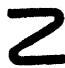
\includegraphics[keepaspectratio]{images/part002_406c0853.jpg}}

It should be remarked that if \(f\) is a bijective uniformly continuous mapping of \(\mathbf{Y}_1\) onto \(\mathbf{Y}_2\) , its extension by continuity need be neither injective nor surjective (Exercise 3).
